\documentclass{article}
\usepackage[utf8]{inputenc}
\usepackage{graphicx}
\usepackage{listings}
\usepackage{float}
\usepackage{indentfirst}
\usepackage{xcolor}
\usepackage{fmtcount}
\usepackage{geometry}
\usepackage{hyperref}

\lstset{basicstyle=\ttfamily\color{blue}}
\newcommand{\code}[1]{\lstinline|#1|}

\geometry{margin=1in}

\title{EEL 4712C - Digital Design: Lab Report 6}
\author{Cole Rottenberg \\ 11062528}
\date{April 29\textsuperscript{th}, 2024}

\lstset{
  language=VHDL,
  numbers=left,
  stepnumber=1,
  tabsize=2,
  numbersep=5pt,
  backgroundcolor=\color{white},
  showspaces=false,
  showtabs=true,
  frame=single,
  rulecolor=\color{black},
  captionpos=b,
  breaklines=true,
  breakatwhitespace=true,
  title=\lstname,
}

\begin{document}

\maketitle

\section*{Lab Report}

\subsection*{Problem Statement}
% Provide a short informal description of the lab’s goals (From the lab assignment)
% If required, specify the system to design.
% - Define the inputs.
% - Define the outputs.
% - Define the function of your system. 
% This section should be 1-2 paragraphs long.
The Goal of the Lab is to explore the use of OSVVM for creating testbenches for VHDL code. The lab will focus on creating a testbench for a simple ALU design. The ALU design will have two 8-bit inputs and an 8-bit output. The ALU will have the following operations: ADD, SUB, AND, OR. The ALU will have an output signal as well as three flags: zero, positive, and negative. The testbench will be used to verify the functionality of the ALU.
\subsection*{Design}
% Describe the design decisions you made.
% - What components did you use?
% - What signals did you use to connect the components?
% - What algorithms did you use?
% Code Segment or block diagrams may be included here.
% Explain your design choices(pros/cons).
% Any designs made in prelab should be included here but more briefly.
% This section should be 1-2 paragraphs long.
The design of the ALU testbench will be based on the OSVVM library. The testbench will be used to verify the functionality of the ALU. The testbench will have a process that will check each bin for an operation and if the coverage is complete. The testbench will run until all the coverages of input opcodes and output flags are met. The testbench will also have a process that will check the output flags and the operations of the ALU. We will have a final process that will generate these random inputs and opcodes for the ALU. The testbench will be used to verify the functionality of the ALU.

\subsection*{Implementation}
% Describe the implementation process.
% Code segments or block diagrams may be included here.
% What time did you need to complete your design?
% This section should be 1-2 paragraphs long.
The implementation followed mostly what the ring\_buffer\_tb did. The testbench was created with the OSVVM library. There were some minor changes due to the lack of a clock within the ALU but overall the testbench matched the one within the example ring\_buffer\_tb. The testbench was able to verify the functionality of the ALU. The testbench was able to verify the functionality of the ALU. The implementation of the testbench can be seen in Listing \ref{lst:alu-tb}.

\subsection*{Testing}
% Describe how you tested your design.
% Did everything work as expected?
% - Did inputs match the expected outputs?
% - Special cases?
% Include if possible, timing diagram of photo/video of the system.
The actual testing of a testbench is a little difficult as it is often difficult to decode whether the ALU is broken or the testbench is broken. In the end the only bit of testing that was overwhelmingly helpful was the coverage data which helped my find a bug in my code regarding the operations using signed datatypes and SLVs.
\subsection*{Conclusions}
% Summarize in one paragraph, the work you did, the success and problems you encountered, and how to improve next in the future.
% This section should only be 1 paragraph long.
This was on of the most helpful labs and I am excited for the opportunity to use OSVVM in the future. The lab was a success and I was able to verify the functionality of the ALU. The only problem I encountered was a bug in my code regarding the operations using signed datatypes and SLVs. In the future I will be more careful with my datatypes and how I use them in my code. 

As seen below in the images, the part 1 testbench was able to compile and simulate. This can be seen in Figures \ref{fig:ex-comp} and \ref{fig:ex-sim}. The ALU testbench was also able to compile and simulate. This can be seen in Figure \ref{fig:alu-sim}.

\section*{Appendix}
% Include all postlab code, screenshots, and simulations here. ALL SIMULATIONS MUST BE ANNOTATED. This means pointing out particularly important parts of a simulation. This can be done with arrows or textboxes. All figures must be captioned. Code should be commented a fair amount.

\begin{figure}[H]
    \centering
    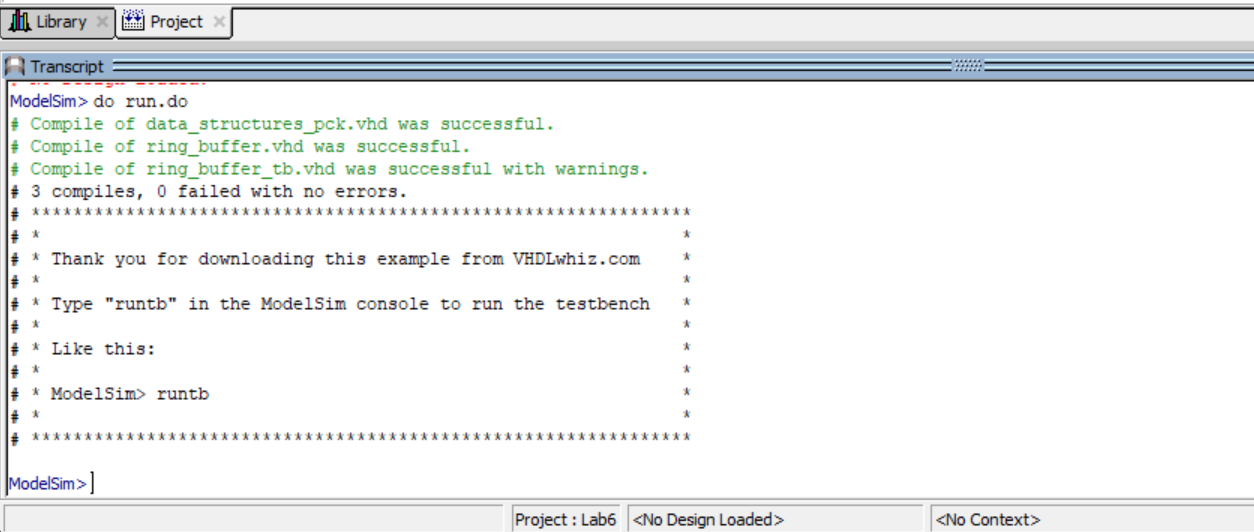
\includegraphics[width=\textwidth]{Part1.png}
    \caption{Testbench Compilation}
    \label{fig:ex-comp}
\end{figure}

\begin{figure}[H]
    \centering
    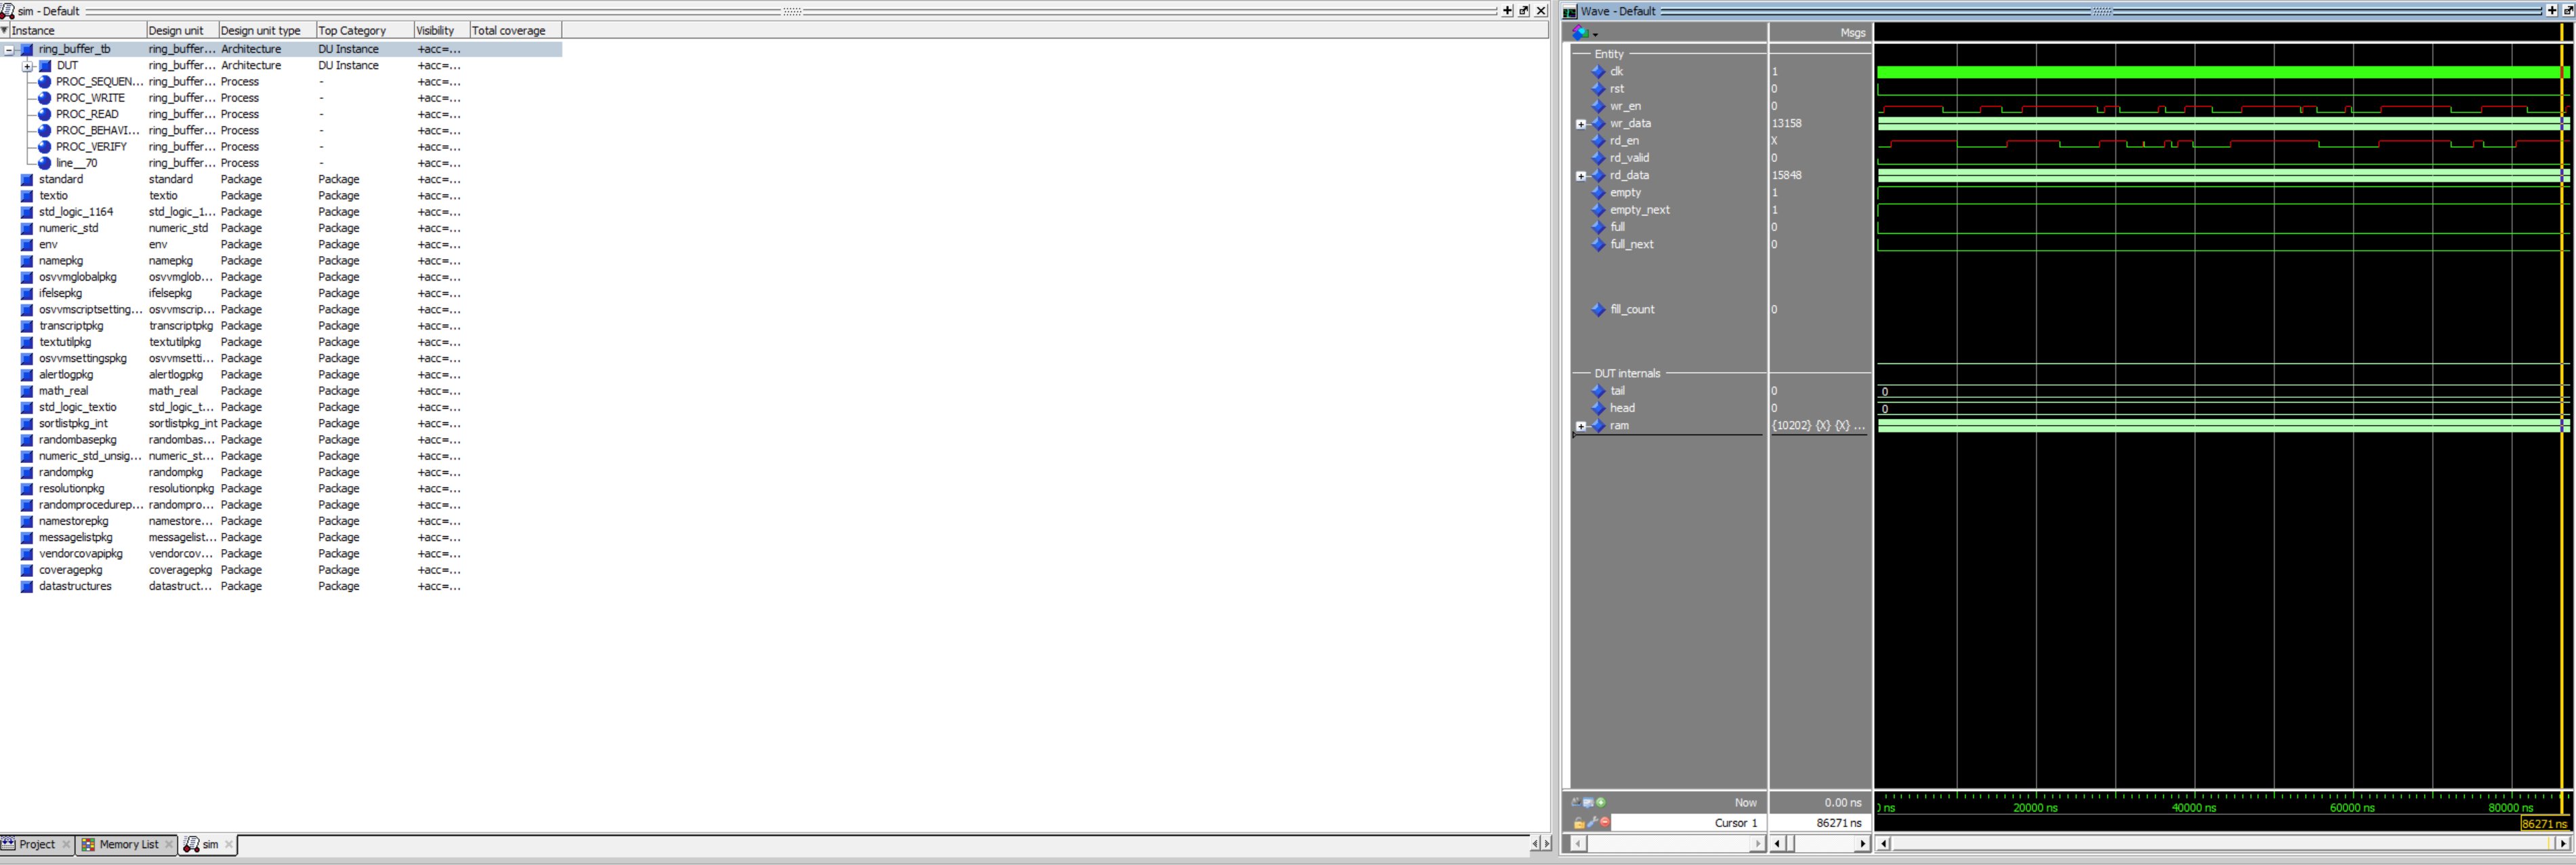
\includegraphics[width=\textwidth]{Part1_TB.png}
    \caption{Testbench Simulation}
    \label{fig:ex-sim}
\end{figure}

\begin{figure}[H]
    \centering
    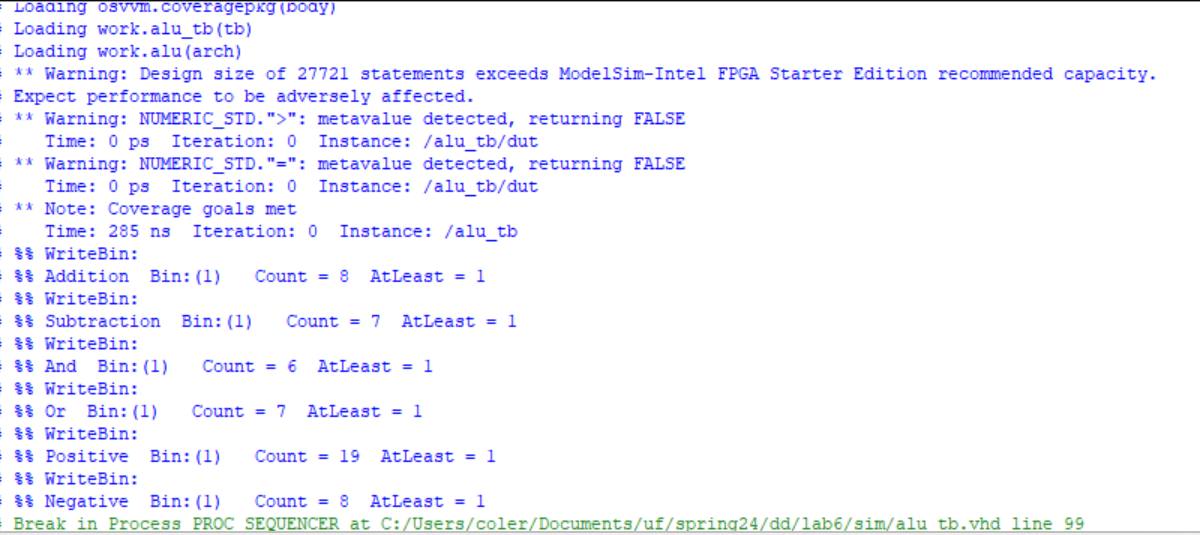
\includegraphics[width=\textwidth]{Part2.png}
    \caption{ALU Testbench Simulation}
    \label{fig:alu-sim}
\end{figure}

\begin{lstlisting}[caption=ALU Testbench, label=lst:alu-tb]
library ieee;
use ieee.std_logic_1164.all;
use ieee.numeric_std.all;

use std.env.finish;

library osvvm;
use osvvm.RandomPkg.all;
use osvvm.CoveragePkg.all;


-- enter your code below
entity alu_tb is 
end alu_tb;

architecture tb of alu_tb is 
  -- ALU signals
  constant clock_period : time := 10 ns;
  signal clk : std_logic := '0';
  -- Inputs
  constant WIDTH : integer := 8;
  signal in0, in1 : std_logic_vector(WIDTH-1 downto 0);
  signal sel : std_logic_vector(1 downto 0);

  -- Outputs
  signal output : std_logic_vector(WIDTH-1 downto 0);
  signal neg : std_logic;
  signal zero : std_logic;
  signal posi : std_logic;

  -- OSVVM Shared Variables
  shared variable rv : RandomPType;
  shared variable bin1, bin2, bin3, bin4, bin5, bin6, bin7 : CovPType; -- 7 coverage bins
begin 
  -- ALU instance
  dut : entity work.alu 
    port map(
      in0 => in0,
      in1 => in1,
      sel => sel,
      output => output,
      neg => neg,
      zero => zero,
      posi => posi
    );

  -- clock generation
  clk <= not clk after clock_period/2;

-- Process sequencer

  PROC_SEQUENCER : process
  begin

    -- Set up coverage bins for the ALU
    bin1.AddBins("Addition", ONE_BIN);
    bin2.AddBins("Subtraction", ONE_BIN);
    bin3.AddBins("And", ONE_BIN);
    bin4.AddBins("Or", ONE_BIN);
    bin5.AddBins("Positive", ONE_BIN);
    bin6.AddBins("Negative", ONE_BIN);
    bin7.AddBins("Zero", ONE_BIN);

    wait until rising_edge(clk);

    loop
      wait until rising_edge(clk);

      -- Collect coverage data for the ALU
      bin1.ICover(to_integer(sel = "00"));
      bin2.ICover(to_integer(sel = "01"));
      bin3.ICover(to_integer(sel = "10"));
      bin4.ICover(to_integer(sel = "11"));
      bin5.ICover(to_integer(posi = '1'));
      bin6.ICover(to_integer(neg = '1'));
      bin7.ICover(to_integer(zero = '1'));

      -- Stop the test when all coverage goals have been met
      exit when
        bin1.IsCovered and
        bin2.IsCovered and
        bin3.IsCovered and
        bin4.IsCovered and
        bin5.IsCovered and
        bin6.IsCovered and
        bin7.IsCovered;
    end loop;
    
    report("Coverage goals met");

    -- Print coverage data
    bin1.WriteBin;
    bin2.WriteBin;
    bin3.WriteBin;
    bin4.WriteBin;
    bin5.WriteBin;
    bin6.WriteBin;
    
    finish;
  end process;

-- Generate Random Values for the ALU
  PROC_RANDOM : process
  begin
    in0 <= std_logic_vector(to_unsigned(rv.RandInt(0, 128), WIDTH));
    in1 <= std_logic_vector(to_unsigned(rv.RandInt(0, 128), WIDTH));
    -- All four possible ALU operations 00, 01, 10, 11
    sel <= std_logic_vector(to_unsigned(rv.RandInt(0, 3), 2));
    
    wait for 10 ns;
  end process;

  -- Emulate the ALU operation
  PROC_BEHAVIORAL_MODEL : process
  -- Variables for the ALU operation
  -- We need to turn the SLVs into  signed
  variable in0_int, in1_int : signed(WIDTH-1 downto 0);
  variable output_int : signed(WIDTH-1 downto 0);

  begin
    in0_int := signed(in0);
    in1_int := signed(in1);
    wait until rising_edge(clk);
    output_int := signed(output);
    case sel is
      when "00" =>
        assert output = std_logic_vector(signed(in0) + signed(in1))
          report "Addition failed"
          severity failure;
      when "01" =>
        assert output = std_logic_vector(signed(in0) - signed(in1)) 
          report "Subtraction failed"
          severity failure;
      when "10" =>
        assert output = std_logic_vector(signed(in0 and in1))
          report "And failed"
          severity failure;
      when "11" =>
        assert output = std_logic_vector(signed(in0 or in1))
          report "Or failed"
          severity failure;
      when others =>
        report "Invalid operation"
          severity failure;
    end case;

    -- Check the ALU flags
    if output_int > 0 then
      assert posi = '1' 
        report "Positive flag failed"
        severity failure;
    end if;
    if output_int < 0 then
      assert neg = '1' 
        report "Negative flag failed"
        severity failure;
    end if;
    if output_int = 0 then
      assert zero = '1' 
        report "Zero flag failed"
        severity failure;
    end if;

  end process;

end tb;

\end{lstlisting}


\end{document}
